\section{分次环的\texorpdfstring{$\proj$}{Proj}}\label{s:3.2}

\subsection{\texorpdfstring{$\proj S$}{Proj S}的构造}\label{s:3.2.1}

到目前为止,非仿射概形最重要的例子是在仿射概形$\spec A$上的\textit{射影}概形,
其中$A$是任意一个交换环。(为简单起见,我们常常说一个概形在$A$上射影,
而不说在$\spec A$上射影。)这样的一个概形来自于一个分次$A$-代数,而构造过程
非常类似于从它的齐次坐标环构造一个射影簇。我们同样可以从一个分次$\oo_B$-代数层
开始,定义在任意的基概形$\spec B$上射影的概形,这个推广有重要的应用。
但对这个理论中的大部分情况而言,我们都可以将情况约化到$B$是一个仿射概形,
故而在这里,我们对一般性的追求也仅止于此。

为了描述这个构造,我们从一个正分次$A$-代数开始,其中$A$是这个代数的$0$次部分,
即一个$A$-代数$S$具有分次
\[
	S=\bigoplus_{\nu=0}^\infty S_\nu\quad \text{(作为$A$-模)}
\]
使得
\[
	S_\nu S_\mu \subset S_{\nu+\mu}\quad \text{以及} \quad S_0=A.
\]
$S$中的一个元素如果处于$S_\nu$中,则它被称为$\nu$-\textit{次齐次}的。我们
将从$S$定义一个$A$-概形$X=\proj S$. 在$A$上射影的概形就被定义为具有形式
$\proj S$的概形,其中$S$是一个有限生成$A$-代数。代数$S$被称为$X$的
\textit{齐次坐标环},尽管(类似于射影簇的齐次坐标环)实际上他并不由$X$所决定。

当$S$是$A$上的多项式环
\[
	S=A[\text{$x_0$, $\dots$, $x_r$}]
\]
时,它具有如下分次:$A$中的元素是零次的,而每一个变量的分次都是$1$,则给出的
概形$\proj S$被称为\textit{$A$上的射影$r$-空间},记作$\mathbb{P}_A^r$.
(后面的习题将说明这个概形与第 \ref{chap:1} 章中定义的概形$\mathbb{P}_A^r$
是相同的。)在$A=K$是一个域的例子中,概形$\mathbb P_K^r$与$K$上的
名为射影空间的簇之间的关系就类似于概形$\mathbb A_K^r$与名为仿射$r$-空间
的簇之间的关系。

简单起见,我们将假设代数$S$在$A$上被它的$1$-次元素所生成,类似于多项式环那样,
一般的情况我们留做习题。(换个推广方向,如果$S$并没有假设在$A$上有限生成,
下面我们说的绝大部分内容依然成立,但这种推广用得相对较少)。

$\proj S$可以如下定义:将$S$中的正次齐次元生成的理想记作
\[
	S_+=\bigoplus_{\mu=1}^\infty S_\mu.
\]
我们称一个理想是\textit{齐次}的如果它由齐次元所生成。底空间$|\proj S|$是环$S$中所有不包含$S_+$的齐次素理想的集合(它们有时候被叫做\textit{相关}素理想,而$S_+$因此被叫做\textit{无关理想})。$|\proj S|$上的拓扑通过闭集定义,闭集取做形如
\[
	V(I):=\{\pp\,|\,\text{$\pp$是$S$的包含$I$的相关素理想}\}
\]
的集合,其中$I$是$S$的齐次理想。

我们将在开集基的每一个元素上明确$|\proj S|$的概形结构。为此,令$f$是$S$的任意$1$-次齐次元素,以及$U$是开集
\[
	|\proj S|-V(f),
\]
即所有不包含$f$的齐次素理想(于是也不包含$S_+$)。$U$中的点可以等同于
$S[f^{-1}]$中的齐次素理想。另一方面,那些对应于环$S[f^{-1}]$中
所有的$0$-次素理想的齐次素理想的集合,我们将其记作$S[f^{-1}]_0$,
见Exercise \ref{exe:3.6}(a). 
于是,我们可以将$U$与拓扑空间$\spec S[f^{-1}]_0$相等同,
然后给他一个相应的仿射概形结构。我们将用$(\proj S)_f$来记这些
$\proj S$的仿射开子概形。如果$1$-次元$x_0$, $x_1$, $\dots$们生成了一个理想,
它的根是无关理想$S_+$,于是开集
\[
	(\proj S)_{x_i}:=\proj S-V(x_i)
\]
就构成了$\proj S$的一个仿射开覆盖。

如果$g$是$S$的另一个$1$-次元,则重叠部分$(\proj S)_f\cap (\proj S)_g$是$(\proj S)_f$的由
\[
	S[f^{-1}]_0[(g/f)^{-1}]=S[f^{-1},g^{-1}]_0
\]
的谱给出的仿射开集。因为上式关于$f$和$g$对称,所以我们有一个自然的等同
\[
	((\proj S)_f)_{(g/f)}=((\proj S)_g)_{(f/g)}.
\]
正如第 \ref{s:1.2.4} 节中讨论的黏合构造,它们将$\proj S$变为了一个概形。

在本节的剩余部分以及下节中,我们将展示一些射影概形的基本事实以及
它们的闭子概形。因为这些事实以及它们的证明与簇的情况中的很类似,
我们将它们留作习题。

% proofread @ 2018.04.01

\begin{exe}\label{exe:3.6}
\begin{compactenum}[(a)]
\item 对$S$任意的齐次理想$I$,以及$1$-次齐次元$f$,交集
\[
	(I\cdot S[f^{-1}])\cap S[f^{-1}]_0
\]
由一族$I$的齐次生成元乘以合适的$f$的(负的)次幂生成
($f$是任意次的推广见 Exercise \ref{exe:3.10})。
于是,$S[f^{-1}]$的齐次素理想一一对应于$S[f^{-1}]$的$0$-次元构成的环的素理想。
对应由$S[f^{-1}]$的素理想$\pp$变为$\mathfrak q=\pp\cap S[f^{-1}]_0$给出,
其逆为将$S[f^{-1}]_0$的素理想$\mathfrak{q}$变为$\mathfrak qS[f^{-1}]$.

\item 令$S=A[x_0$, $\dots$, $x_r]$为多项式环,
而$U$是$\mathbb P_A^r=\proj S$的仿射开集$(\mathbb P_A^r)_{x_i}$. 由定义,
\[
	U=\spec S[x_i^{-1}]_0,
\]
证明
\[
	S[x_i^{-1}]_0=A[x'_0,\dots,x'_r]
\]
为生成元$x'_j=x_j/x_i$的多项式环。(
注意$x'_i=1$,所以这是一个$r$变量的多项式环。)于是
\[
	(\mathbb P^r_A)_{x_i}=\mathbb A_A^r
\]
所以射影$r$-空间被$r+1$个仿射$r$-空间所覆盖,
就像第 \ref{chap:1} 章中所描述的那样。

\item 考虑一个映射$\alpha:S\to S[x_i^{-1}]_0$,
他将$x_i$变为$1$以及对$j\neq i$将$x_j$变为$x'_j$. 
从(a)证明如果$I$是$S$的一个齐次理想,于是
\[
	I':=I\cdot S[x_i^{-1}]\cap S[x_i^{-1}]_0=\alpha(I)'\cdot S[x_i^{-1}]_0.
\]
从$I$构造$I'$的过程被称为\textit{非齐次化}。
像经典的那样,描述与其相反的过程,齐次化。
\end{compactenum}
\end{exe}

\begin{exe}\label{exe:3.7}
如果$I$是一个分次环$S$的齐次理想,我们有一个底空间的包含
\[
	|\proj S/I|\subset |\proj S|.
\]
证明,这个子集与一个仿射开集$(\proj S)_f$的交集是$(\proj S)_f$的一个闭子集,
所以$\proj S/I$能被看作$\proj S$的一个闭子概形。
每个由$1$-次元有限生成的$A$-代数是某个多项式环
$A[x_0$, $\dots$, $x_r]$模掉一个齐次理想得到的商环,
所以我们看到\textit{每个$A$上的射影概形是一个$A$上的射影空间的闭子概形}。
下面我们将在Exercise \ref{exe:3.15} 和 \ref{exe:3.16} 具体看到环$S$的理想
与$\proj S$的闭子概形之间的联系。
\end{exe}

\begin{exe}\label{exe:3.8}
证明$\mathbb P_A^r$是开集$\mathbb A_A^{r-1}$与闭集$\mathbb P_A^{r-1}$
的不交并。特别地,$\mathbb P^0_A=\spec A$. 所以比如,
我们能将$\mathbb P_{\mathbb Z}^1$看成$\zz$上的仿射直线$\mathbb A_\zz^r$
(如第 \ref{chap:2} 章的图)与一个同构于$\spec \zz$的“无穷远点”的并,
如下图所示

\begin{center}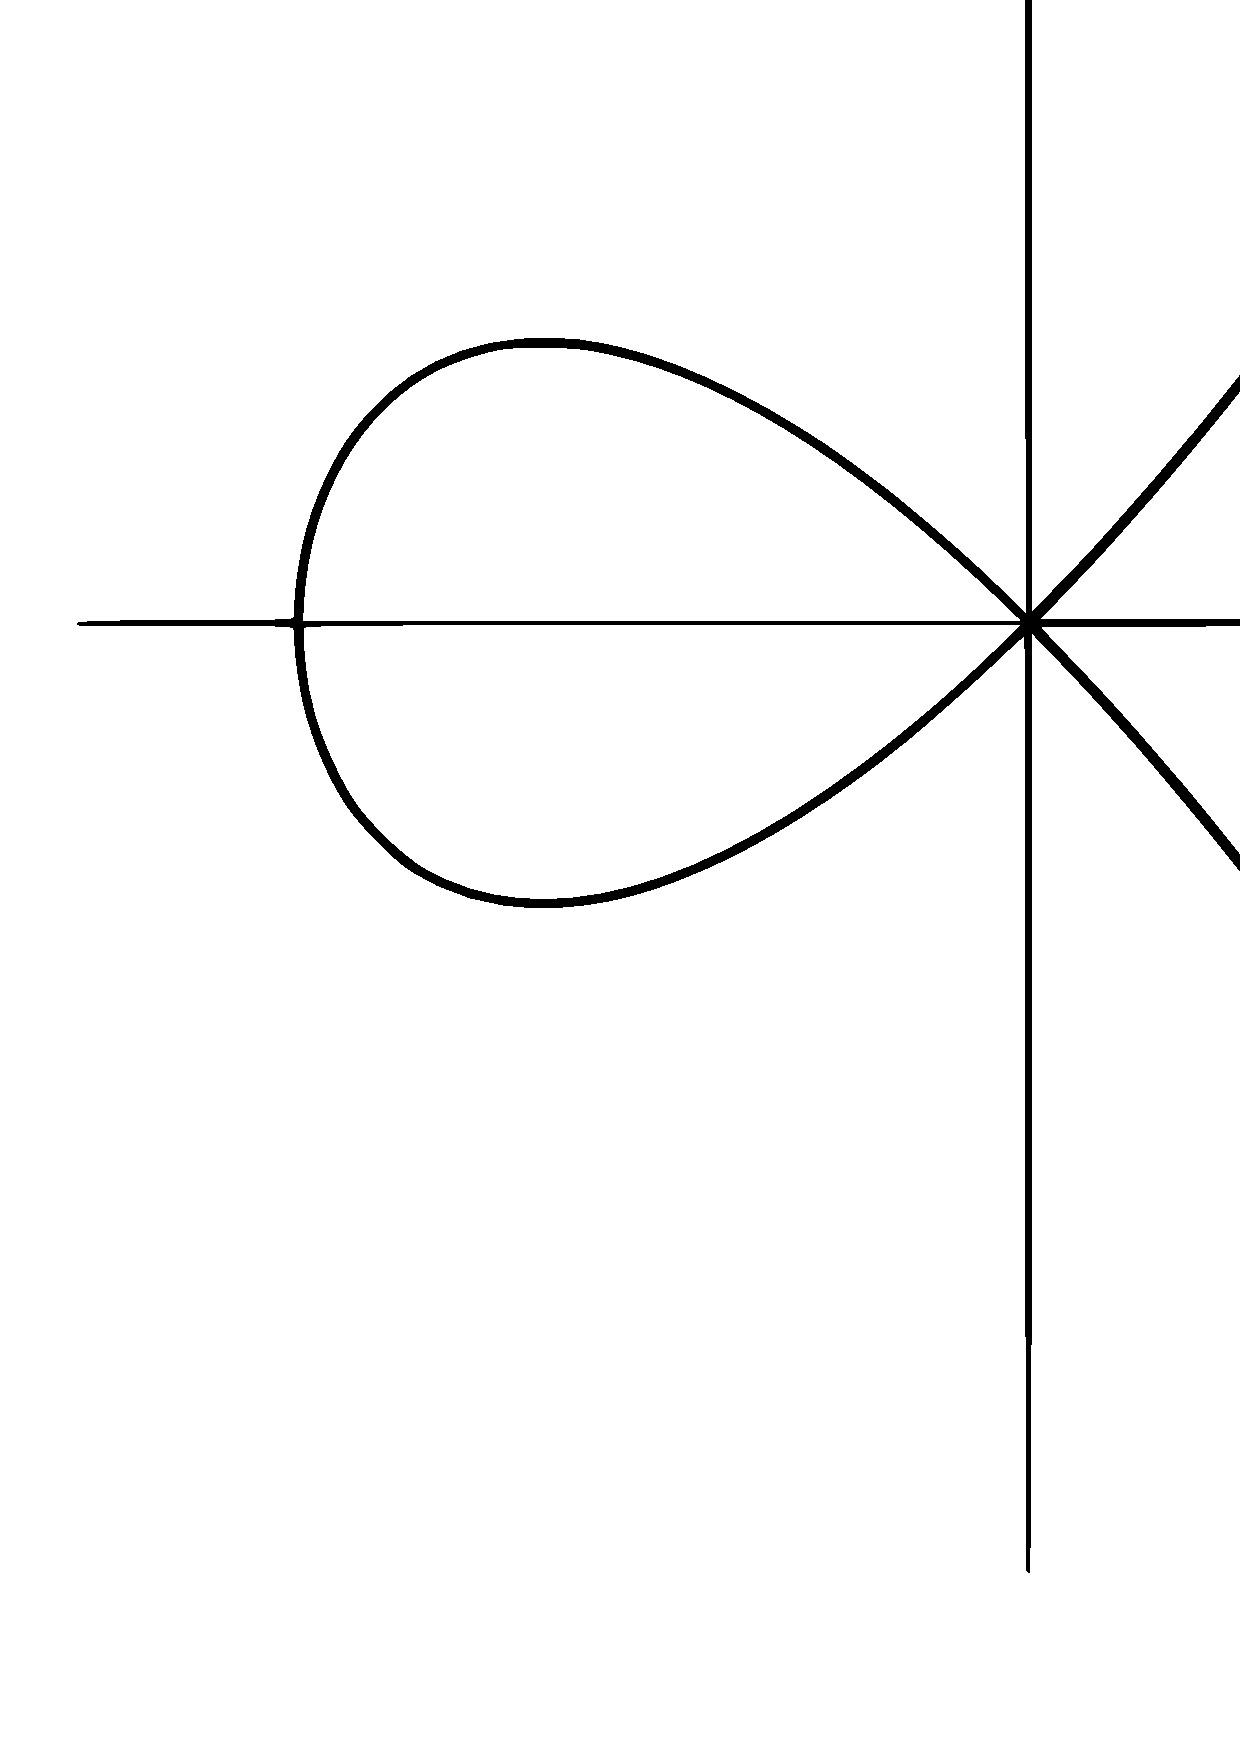
\includegraphics[scale=\scale,bb=0 0 668 462]{\PICDIR/2.png}\end{center}
\end{exe}

\begin{exe}\label{exe:3.9}
在上图中添入点$(4x_1-5x_0)$, $(2x_1-5x_0)$以及$(5)$的闭包
(可以与第 \ref{s:2.4.3} 节中的$\mathbb A_{\mathbb Z}^2$的图相比较)。
\textit{注意}:曲线$(4x_1-5x_0)$应该画得与“无穷远点”$(x_0)$相切,
而曲线$(2x-5x_0)$不能。通俗地,我们可以说这是因为函数$5/4$在$(2)$
处有一个双极点,而$5/2$只有一个单极点。
(同样可见 Exercise \ref{exe:2.38} 中的讨论。)
\end{exe}

\begin{exe}\label{exe:3.10}
按上面的记号,令$h$为$S$的一个正次齐次元。集合
\[
	(\proj S)_h:=\proj S-V(h)
\]
同前为$S$中不包含$h$的齐次素理想构成的集合。
证明这个集合依然一一对应于$S[h^{-1}]_0$的素理想,
所以实际上存在一个$\spec S[h^{-1}]_0$与$\proj S$的(仿射)开子概形的同构。同样证明,这样的仿射开集族
\[
	\{(\proj S)_h\}_{h\in H}
\]
是一个$\proj S$的开覆盖,当且仅当$H$的元素生成了一个根为$S_+$的理想。
\end{exe}

\begin{exe}\label{exe:3.11}
推广$\proj S$的定义到$S$不被$1$-次元所生成的情况,以及证明$\proj S$是一个射影概形。
\end{exe}

\begin{exe}\label{exe:3.12}
令$S$是一个分次环,没必要是有$1$-次元生成的。
对任意的正次$d$,定义$S$的$d$-次\textit{Veronese 子环}为分次环
\[
	S^{(d)}=\bigoplus_{\nu=1}^\infty S_{d\nu}
\]
证明$\proj S$同构于$\proj S^{(d)}$. 
然而,证明如果$S=A[x,y]$,则$S^{(d)}$作为分次代数(甚至仅作为环)并不同构于$S$. 
于是,就像在簇中那样,分次代数与射影概形的对应并不是一一的。
\end{exe}

\subsection{\texorpdfstring{$\proj R$}{Proj R}的闭子概形}\label{s:3.2.2}

一个齐次理想$I\subset A[x_0$, $\dots$, $x_r]$确定了一个凝聚理想层$\tilde I\subset \mathscr O_{\mathbb P_A^r}$,因而一个$\mathbb P_A^r$的闭子概形。下面的习题建立了这些事实。

\begin{exe}\label{exe:3.13}
对每个开集
\[
	U_i=(\mathbb P_A^r)_{x_i}=\spec A[x_0,\dots,x_r,x_i^{-1}]_0\cong \mathbb A_A^r,
\]
令$\tilde I(U_i)$为理想$I\cdot A[x_0,\dots,x_r,x_i^{-1}]\cap A[x_0,\dots,x_r,x_i^{-1}]_0$. 证明这个定义可以以唯一的方式扩张到其他开集$U$上使得$\tilde{I}$成为一个凝聚理想层。所以我们称$\mathbb P_A^r$的闭子概形$V(\tilde{I})$\textit{关联于一个齐次理想$I$}.
\end{exe}

\begin{exe}\label{exe:3.14}
反之,给定一个$\mathbb P_A^r$的一个闭子概形,我们可以定义一个齐次理想$I(X)\subset A[x_0$, $\dots$, $x_r]$,它是齐次多项式$p(x_0,\dots,x_r)$生成的理想,其中齐次多项式需满足对每一个$i$,将其置于$1$后给出了元素
\[
	p(x_0,\dots,1,\dots,x_r)\in \mathscr I_X(U_i)\subset A[x_0,\dots,x_r,x_i^{-1}]_0.
\]
证明,如果$I=I(X)$,则$\tilde I=\mathscr I_X$.
\end{exe}

注意到连同 Exercise \ref{exe:3.7} ,它说明了每一个射影簇的闭子概形也是射影的:如果$I\subset S=A[x_0$, $\dots$, $x_r]$是一个齐次理想,则$V(\tilde{I})\subset \mathbb P^r_A$同构于概形$\proj S/I$.

\begin{exe}\label{exe:3.15}
子概形与理想的对应不再像仿射概形的情况是一一对应了。比如,证明在$\mathbb P_K^1$中,其中$K$是一个域,理想$I=(x_0)$和$I'=(x_0^2,x_0x_1)$都定义了同一个约态、单点子概形。更一般地,证明,如果$I\subset S=K[x_1$, $\dots$, $x_r]$是任意的齐次理想,以及对任意的整数$n_0$,通过
\[
	I'=\bigoplus_{n\geq n_0}I_n
\]
定义一个理想$I'\subset I$,则$I$和$I'$定义了$\mathbb P_K^r$的同一个子概形。
\end{exe}

\begin{exe}\label{exe:3.16}
为了解决这点,定义一个齐次理想$J\subset S:=A[x_0$, $\dots$, $x_r]$的\textit{饱和化}为理想
\[
	I=\{F\in S\,:\, \text{对某个$n$,$F\cdot S_n\subset J$}\},
\]
以及,称一个齐次理想是\textit{饱和}的,如果它等于它的饱和化。证明,存在一个$\mathbb P_A^r$的子概形与饱和理想之间的一一对应。
\end{exe}

\begin{exe}\label{exe:3.17}
证明,Exercise \ref{exe:3.12} 中的同构定义了一个射影空间$\mathbb P_A^r$以及$\mathbb P_A^N$的一个闭子概形之间的同构,其中$N=\dim_A(A[x_0$, $\dots$, $x_r]_d)$.(这就是概形版的Veronese映射。)
\end{exe}

\begin{exe}\label{exe:3.18}
证明,如果$R$是一个环$A=R_0$上的有限生成分次环(没必要是由其$1$-次元生成的),$\proj R$同构于某个射影空间$\mathbb P_A^r$的闭子概形。
\end{exe}

我们以一个定义和基本定理结束这一小节。

\begin{defi}
一个概形间态射$\varphi:X\to Y$被称为\textit{射影}的,如果他是一个闭嵌入$X\to \mathbb P_Y^n$和结构态射$\mathbb P_Y^n\to Y$的复合。
\end{defi}

注意到,如果$Y=\spec A$是仿射的,这相当于说$X$具有形式$\proj S$,其中$S$是一个有限生成$A$-代数。射影态射的基本事实前面已经说过了:

\begin{thm}\label{thm:3.20}
射影态射是逆紧的。
\end{thm}

证明可见Hartshorne [1977, Theorem II.4.9].

\begin{exe}\label{exe:3.21}
证明,有限态射$\varphi:X\to Y$是逆紧的且局部射影的,所谓局部射影即指,
$Y$可以被开集族$U\subset Y$所覆盖,使得限制$\varphi:V=\varphi^{-1}U\to U$
是射影的。(我们采用了 Hartshorn [1977, Section II.4] 中射影态射的定义,
而在 Grothendieck [1961, EGA II, 5.5] 中,
射影是指我们这里被叫做局部射影的性质。)
\end{exe}

\subsection{整体\texorpdfstring{$\proj$}{Proj}} \label{s:3.2.3}

\paragraph*{分次\texorpdfstring{$\oo_X$}{OX}-代数层的\texorpdfstring{$\proj$}{Proj}}\addcontentsline{toc}{subsubsection}{分次\texorpdfstring{$\oo_X$}{OX}-代数层的\texorpdfstring{$\proj$}{Proj}}
分次环$S$的$\proj$的构造给出了一个概形$X=\proj S$以及一个结构态射
$X\to B=\spec(S_0)$. 因为$\proj S$与$S$的关联是函子性的,
所以存在一个更一般的构造,给出概形$X$以及结构态射$X\to B$,
其中$B$是任意概形,使得当$B$是仿射的时候将回到$\proj$:对一般的$B$,
我们只需用$\oo_B$上的代数层代替分次$S_0$-代数$S$.

为实现这个构造,令$B$为任意概形,一个\textit{拟凝聚分次$\oo_B$-代数层}
是指一个$B$上的拟凝聚代数层$\mathscr F$,具有一个分次
\[
	\mathscr F=\bigoplus_{\nu=0}^\infty \mathscr F_\nu
\]
使得$\mathscr F_\nu \mathscr F_\mu\subset \mathscr F_{\mu+\nu}$
以及$\mathscr F_0=\oo_B$. 因此,对每一个仿射开集$U\subset B$,
其坐标环为$A=\oo_B(U)$,环$\mathscr{F}(U)$是一个分次$A$-代数,
其$0$-次部分为$\mathscr F(U)_0=A$. 

给定这样一个层$\mathscr F$,对每个仿射开集$U\subset B$,
我们令$X_U\to U$为概形$X_U=\proj \mathscr F(U)$及结构态射
$\proj \mathscr F(U)\to \spec A=U$. 对每个$B$的开子集的含入$U\subset V$,
限制映射$\mathscr F(V)\to \mathscr F(U)$是一个分次环的同态,
其$0$-次部分为限制映射$\oo_B(V)\to \oo_B(U)$,
所以诱导了一个映射$X_U\to X_V$与结构态射$X_U\to U$和$X_V\to V$以及
含入$U\hookrightarrow V$可交换。我们于是可以将概形$X_U$粘起来得到概形
$X$,其具有结构态射$X\to B$,记作$\proj \mathscr F$,
而$X$的构造则被称为\textit{整体$\proj$}.

就像在普通的$\proj$中一样,大部分情况下代数层$\mathscr F$由其$1$-次部分$\mathscr F_1$所生成,以及$\mathscr F_1$是凝聚的(或者,某种程度上更一般地,对某个$d>0$,Veronese 子层
\[
	\mathscr F^{(d)}=\bigoplus_{\nu=0}^\infty \mathscr F_{d\nu}
\]
由$\mathscr F_{d\nu}$所生成,而$\mathscr F_{d\nu}$是凝聚的
)。在这个假设下,同样如同普通的$\proj$,态射$\proj \mathscr F\to B$是逆紧的。

整体$\proj$最简单的例子给了我们任意概形$S$上的射影空间的另一个构造。回忆在第 \ref{chap:1} 章,任意概形$S$上的射影空间是黏合构造而成的:如果$S$被仿射概形族$U_\alpha=\spec R_\alpha$所覆盖,我们定义射影空间$\mathbb P_S^n$为射影空间$\mathbb P_{U_\alpha}^n$的并,并通过$U_\alpha\cap U_\beta$上的恒等映射诱导的黏合映射粘起来。此外,我们也可以通过乘积来定义它:
\[
	\mathbb P_S^n=\mathbb P_{\mathbb Z}^n\times_{\spec \mathbb Z}S.
\]
最后,我们可以将其实现为$S$上秩为$n+1$的自由层的对称代数的整体$\proj$:

\begin{exe}\label{exe:3.22}
令$S$为任意概形。证明$S$上的射影空间$\mathbb P_S^n$可以由整体$\proj$构造:
\[
	\mathbb P_S^n=\proj \left(\operatorname{Sym}(\oo_S^{\oplus n+1})\right).
\]
\end{exe}

特别地,在纤维积外,我们可以通过整体$\proj$来实现给定概形$S$上的射影空间的乘积:如果我们记$\oo_{\mathbb P_S^r}[X_0$, $\dots$, $X_m]$为分次$\oo_{\mathbb P_S^n}$-代数层$\operatorname{Sym}\left(\oo_{\mathbb P_S^n}^{\oplus m+1}\right)$,则
\[
	\mathbb P^n_S\times_S \mathbb P^m_S=\proj \oo_{\mathbb P^n_S}[X_0,\dots,X_m].
\]
第三种方式是通过\textit{Segre嵌入}:

\begin{exe}\label{exe:3.23}
令$S$为任意概形。证明
\begin{align*}
\mathbb P_S\times_S \mathbb P_S^m &\cong V\left(\{X_{i,j}X_{k,l}-X_{i,l}X_{k,j}\}\right)\subset \proj \oo_S[\{X_{i,j}\}_{0\leq i\leq n;0\leq j\leq m}]\\
& = \mathbb P_S^{(n+1)(m+1)-1}.
\end{align*}
\end{exe}

于是,至少局部地在基上,这给了我们一种方式来描述这样乘积的子概形:

\begin{exe}\label{exe:3.24}
令$S=\spec R$为任意的仿射概形。证明
\[
	X\subset \proj R[x_0,\dots,x_n]\times_S \proj R[y_0,\dots,y_m]=\mathbb P^n_S\times_S\mathbb P^m_S
\]
任意的闭子概形都可以由族$\{F_\alpha(x_0$, $\dots$, $x_n;y_0$, $\dots$, $y_m)\}$的零点集给出,其中$F_{\alpha}$是两族变量$(x_0$, $\dots$, $x_n)$和$(y_0$, $\dots$, $y_m)$的齐次函数。特别地,证明矩阵
$
\begin{pmatrix}
x_0&x_1&\cdots &x_n\\
y_0&y_1&\cdots &y_n\\
\end{pmatrix}
$
的$2\times 2$子式的理想定义了$\mathbb P^n_S\times_S\mathbb P^m_S$中的对角集。推出任意射影态射都是可分的。
\end{exe}

整体$\proj$构造的一个更严肃的应用是定义概形$X$沿着闭子概形$Y\subset X$的\textit{爆破},我们将在第 \ref{chap:5} 章中完整地讨论它。整体$\proj$另一个通常的应用是我们下面描述的矢量丛的射影化。

\paragraph*{凝聚层\texorpdfstring{$\mathscr E$}{E}的射影化\texorpdfstring{$\mathbb P(\mathscr E)$}{P(E)}}\addcontentsline{toc}{subsubsection}{凝聚层\texorpdfstring{$\mathscr E$}{E}的射影化\texorpdfstring{$\mathbb P(\mathscr E)$}{P(E)}}
在 Exercise \ref{exe:3.22} 中看到,概形$S$上的射影空间$\mathbb P_S^n$是$\proj(\operatorname{Sym}(\oo_S^{\oplus n+1}))$. 我们将对任意凝聚层$\mathscr E$做一个类似的构造,定义$\mathscr E$的\textit{射影化}$\mathbb P(\mathscr E)$为$B$-概形
\[
	\mathbb P(\mathscr E)=\proj(\operatorname{Sym} \mathscr E)\to B.
\]

检查最简单的情况,令$V$是域$K$上的$n$-维矢量空间,看成单点概形$\spec K$上的一个矢量丛。$V$的射影化是一个$K$上的维数为$n$的射影空间,而$V^*$的射影化被称为$\mathbb PV$的\textit{对偶射影空间}。$\mathbb P(V)$的$K$-值点对应于$V$的一维商空间,或者等价地,$V$中的超平面。$\mathbb P(V^*)$的$K$-值点对应于$V$的一维子空间,这就是被经典地记作$\mathbb P^n$的射影空间。

一般些,如果$\mathscr E$是一个秩为$n+1$的局部自由层,则$\mathbb P(\mathscr E)$为$B$上的一个\textit{射影丛},即对足够小的仿射开集$U\subset B$,$U$在$\mathbb P(\mathscr E)$中的原像作为$U$-概形同构于射影空间$\mathbb P_U^r$. (如果$\mathscr E$不是局部自由的,则概形$\mathbb P(\mathscr E)$是怎么样的就没那么清楚了。)当$B$是一个代数闭域$K$上的簇,而$\mathscr E$是一个$B$上的矢量丛$E$的截面层,则$\mathbb P(\mathscr E^*)$的$K$-值点对应于$\mathscr E$的纤维的一维子空间,而$\mathbb P(\mathscr E)$的$K$-值点对应于$\mathscr E$的纤维的一维商空间,或等价地,纤维中的超平面。

注意到,任意闭子概形$X\subset \mathbb P_B^n$能被实现为$\proj(\mathscr F)$,其中$\mathscr F$是一个分次$\oo_B$-代数的拟凝聚理想层。更一般地,如果$\mathscr E$是任意凝聚层,则其射影化的任意闭子概形$X\subset \mathbb P(\mathscr E)$也可以如此实现。反之,如果$\mathscr F$是分次$\oo_B$-代数的任意拟凝聚理想层,由$\mathscr F_1$生成,则满射$\operatorname{Sym}(\mathscr F_1)\to \mathscr F$给出了嵌入$X=\proj \mathscr F\hookrightarrow \mathbb P(\mathscr F_1)$.

\begin{exe}\label{exe:3.25}
	令$K$是一个域,$\mathbb P_K^2=\proj K[X,Y,Z]$是$K$上的射影平面,$(\mathbb P_K^2)^*=\proj K[A,B,C]$是对偶射影平面。令$\Sigma$是$(\mathbb P_K^2)^*$上的万有直线,即
	\[
		\Sigma=V(AX+BY+CZ)\subset \mathbb P_K^2\times_K (\mathbb P_K^2)^*
	\]
	看作$(\mathbb P_K^2)^*$上的族。证明,$\Sigma\to (\mathbb P_K^2)^*$是$(\mathbb P_K^2)^*$上的秩为$2$的局部自由层$\mathscr E$,并描述$\mathscr E$.
\end{exe}

\begin{exe}\label{exe:3.26}
	令$B$是任意概形,$\mathscr E$是一个$B$上的局部自由层,以及$E=\spec (\operatorname{Sym}\mathscr E^*)\to B$是$\mathscr E$对应的矢量丛的全空间。证明,我们可以将$E\to B$完备为一个$B$上的射影空间的从:确切地,证明,我们有一个$E$上的含入,到$\mathbb P(\mathscr E^*\oplus \oo_B)$作为其开子概形,补是一个超平面丛$\mathbb P(\mathscr E^*)\subset \mathbb P(\mathscr E^*\oplus \oo_B)$.
\end{exe}


\subsection{切空间和切锥} \label{s:3.2.4}
\paragraph*{仿射与射影切空间}\addcontentsline{toc}{subsubsection}{仿射与射影切空间}
概形的Zariski切空间是抽象矢量空间,但当一个域$K$上的概形$X$被嵌入到一个环绕空间中,比如仿射或射影$K$-空间,我们可以将$X$的一个剩余类域为$K$的点$p$关联于一个对应仿射或者射影空间的线性子簇,其被称为$X$在点$p$的\textit{仿射切空间}或\textit{射影切空间}。在仿射概形$X=V(f_1,\dots,f_k)\subset \mathbb A_K^n$以及点$p=(a_1,\dots,a_n)\in X$的情况中,这是一个由
\[
	V\left(\left\{
		\sum_i \frac{\partial f_\alpha}{\partial x_i}(\alpha_1,\dots,\alpha_n)\cdot (x_i-a_i)
	\right\}_{\alpha=1,\dots,k}
	\right)
\]
给出的子簇。为理解这个概形与Zariski切空间之间的关系,注意到域$K$上的一个矢量空间与仿射空间$\mathbb A_K^n$并不是同一个东西。但是,给定$K$上的一个$n$-维矢量空间$V$,我们可以对$V$给出一个概形$\overline{V}$,它同构于仿射开集$\mathbb A_K^n$,所以$\overline{V}$中剩余类域为$K$的点自然地对应于$V$中的矢量:$\overline{V}$就是对偶空间对称代数的谱
\[
	\overline{V}=\spec (\operatorname{Sym}(V^*)).
\]
我们将称$\overline{V}$为\textit{关联于矢量空间$V$的概形}。

这告诉我们,与域$K$上的仿射空间$\mathbb A_K^n$在$K$-有理点$p\in \mathbb A^n_K$(即一个剩余类域为$\kappa(p)=K$的闭点)的Zariski切空间相关联的概形$\overline{T_p(\mathbb A^n_K)}$,可以自然等同于仿射空间本身,它将$T_p(\mathbb A_K^b)$的原点变成了$p$. 现在,假设$X\subset \mathbb A_K^n$是任意的子概形,$p\in X$是任意的$K$-有理点。含入$\iota:X\hookrightarrow \mathbb A_K^n$在点$p$处的微分$d\iota_p$将Zariski切空间$T_p(X)$表为一个矢量子空间
\[
	d\iota_p:T_p(X)\hookrightarrow T_p(\mathbb A_K^n).
\]
我们取概形的诱导含入
\[
	\overline{d\iota_p}:\overline{T_p(X)}\hookrightarrow
	\overline{T_p(\mathbb A_K^n)}=\mathbb A_K^n
\]
复合上平移态射$t_p:\mathbb A^n_K\to \mathbb A^n_K$,它将原点映射为$p$,得到一个含入
\[
	t_p\cdot \overline{d\iota_p}:\overline{T_p(X)}\hookrightarrow
	\mathbb A_K^n \longrightarrow \mathbb A_K^n.
\]
这个含入的像是$\mathbb A_K^n$的一个仿射子空间,我们将其称为$X$在点$p$的\textit{仿射切空间}。再一次注意到,这是一个概形不是一个矢量空间。

对射影概形$X\subset \mathbb P_K^n$的剩余类域为$K$的点$p$,我们可以类似地关联于一个线性子空间$\mathbb T_p(X)\subset \mathbb P_K^n$. 一种实现它的方式是找一个包含$p$的开子集$U\cong \mathbb A_K^n\subset \mathbb P^n_K$,然后取$X\cap U$在点$p$的仿射切空间在$\mathbb P_K^n$中的闭包。但,我们也有另一种更内蕴的方式。首先,我们记环绕射影空间$\mathbb P_K^n$为关联于矢量空间$V$的射影空间$\mathbb PV$,即是
\[
	\mathbb P_K^n=\proj S
\]
其中
\[
	S=\operatorname{Sym}V^*
\]
是$V$的对偶空间的对称代数。因此,$S_1=V$的$(k+1)$-维线性子空间对应于$\mathbb P_K^n$中的$k$-平面。我们令
\[
	I=I(X)\subset S
\]
为$X\subset \mathbb P_K^n$的齐次理想,以及令$\mm=\mm_p\subset S$为在点$p\in X$为零的形式(form)构成的理想。令$J$是理想$I+\mm^2\subset S$的饱和化。我们定义$X$在点$p$的射影切空间$\mathbb T_p(X)$为$\mathbb P_K^n$的子空间
\[
	\mathbb T_p (X)=V(J\cap S_1)\subset \mathbb P^n_K.
\]
稍加解释:注意到$J$是$p$在$X$中的一阶邻域的理想,即为$X$与$p$的理想$\mm$的平方定义的“丰满点”$P\subset \mathbb P_K^n$的交。于是,射影切空间$\mathbb T_p(X)=V(J\cap S_1)$就是由这个一阶邻域$V(J)$张成的,即是包含$V(J)$的$\mathbb P_K^n$的最小线性子空间。

\begin{exe}\label{exe:3.27}
	证明这个定义与前面的一开始说的\naive 定义一致。
\end{exe}

因为射影概形$X$在$K$-有理点$p\in X$处的射影切空间$\mathbb T_p(X)$是一个环绕射影空间$\mathbb PV$的一个线性子空间,具有形式$\mathbb T_p(X)=\mathbb PW$,其中$W$是一个商矢量空间$V\to W\to 0$. 然后,我们可能问矢量空间$W$与Zariski切空间$T_p(X)$之间具有什么联系。在第 \ref{s:6.2.1} 节中,我们将看到答案是一个正合列
\[
	0\longrightarrow K\longrightarrow W^* \longrightarrow T_p(X)\longrightarrow 0.
\]
更明确一些,如果$V\to U\to 0$是$V$的一个$1$-维商空间,关联于点$p\in X\subset \mathbb PV$,则满射$V\to U$可以经由满射$\varphi:W\to U$分解,进而我们有一个自然的等同
\[
	T_p(X)=\Hom(\operatorname{Ker}\varphi,U).
\]
无论如何,注意到我们都有一个$\mathbb T_p(X)$中经过$p$的直线的集合与$T_p(X)$中经过原点的直线的集合之间的自然等同。

\begin{exe}\label{exe:3.28}
	令$X=V(F)\subset \mathbb P_K^n$是$\mathbb P_K^n$中的超平面,由齐次多项式$F(Z_0,\dots,Z_n)$给出,再令$p=[a_0,\dots,a_n]\in X$是任意一个剩余类域为$K$的点。证明,射影切空间$\mathbb T_p(X)$就是零点集$V(L)\subset \mathbb P_K^n$,其中$L$是线性多项式
	\[
		L(Z_0,\dots,Z_n)=\sum_{k=1}^n\frac{\partial F}{\partial Z_i}(a_0,\dots,a_n)\cdot Z_k.
	\]
\end{exe}

\paragraph*{切锥}\addcontentsline{toc}{subsubsection}{切锥}
对概形$X$在点$p\in X$的切向表现的更准确描述是它的切锥。为定义它,令$X$为任意的概形,$p\in X$是一个点,$\mathscr O_{X,p}$是$X$在点$p$的局部环,以及$\mm=\mm_{X,p}\subset \mathscr O_{X,p}$是$\mathscr O_{X,p}$的极大理想。我们定义$X$在点$p$的\textit{切锥}$TC_p(X)$为概形
\[
	TC_p(X)=\spec \left(\bigoplus_{\alpha=0}^\infty \mm^\alpha/\mm^{\alpha+1}\right).
\]
这个构造的一些简单观察如下。首先,注意到分次环$B=\bigoplus (\mm^\alpha/\mm^{\alpha+1})$由它的$1$-次分次部分
\[
	B_1=\mm/\mm^2=(T_pX)^*
\]
所生成的,因此,$B$是环
\[
	A=\operatorname{Sym}((T_pX)^*)
\]
的商环。我们于是有了一个含入
\[
	TC_p(X)=\spec B\hookrightarrow \spec A=\overline{T_pX},
\]
或者说,$X$在点$p$的切锥自然地是$X$在点$p$的Zariski切空间$T_pX$对应的概形的子概形。

为给出一个更切实的切锥实现,假设$X$是一个域$K$上的仿射空间的子概形,即
\[
	X\subset \spec K[x_1,\dots,x_n],
\]
再令$I=I(X)\subset K[x_1,\dots,x_n]$是$X$的理想;进一步假设点$p\in X$是原点$(x_1,\dots,x_n)\in \mathbb A_K^n$. 对任意的多项式$f\in K[x_1,\dots,x_n]$,记
\[
	f(x_1,\dots,x_n)=f_m(x_1,\dots,x_n)+f_{m+1}(x_1,\dots,x_n)+\cdots,
\]
其中$f_l(x_1,\dots,x_n)$是$l$次齐次多项式以及$f_m\neq 0$;首个非零项$f_m(x_1,\dots,x_n)$被称为$f$的\textit{领头项}%
\footnote{译者注:英文是leading term,大概也可以称为首项?好像不太合适}%
。于是,我们有如下诠释:

\begin{exe}\label{exe:3.29}
	证明切锥
	\[
		TC_p(X)\subset \overline{T_pX}\subset \overline{T_p(\mathbb A_K^n)}=\mathbb A_K^n
	\]
	是由所有多项式$f\in I$的领头项的零点集定义的子概形。
\end{exe}

回到一般的情况,注意到因为环$B=\bigoplus (\mm^\alpha/\mm^{\alpha+1})$是分次的,我们可以同样对$(X,p)$关联一个几何对象$\proj B$. 这是$X$在点$p$的Zariski切空间对应的射影空间$\mathbb P(T_p X)\cong \mathbb P^n_{\kappa(p)}$的一个子概形,称作在$X$在点$p$的\textit{射影化切锥},记作$\mathbb PTC_p(X)$. 在许多情况中,处理作为射影概形以及比切锥少一维的射影化切锥会更方便,但一般来说,他比切锥所包含的信息稍少一些(就像下面的Exercise \ref{exe:3.30} 将展示的,切锥$TC_p(X)$可能在原点有一个嵌入点,而射影化切锥没有)。

尽管,射影空间一般的子概形的度将在第 \ref{s:3.3.1} 节中才定义,我们将在这里提出一个可以由$X$在点$p$的射影化切锥定义的概形不变量:定义$X$在点$p$的\textit{重数}为射影化切锥$\mathbb PTC_p(X)\subset \mathbb P(T_p X)\cong \mathbb P^n_{\kappa(p)}$的度。这个定义展现了另一个例子,告诉我们为何概形会在处理簇时自然出现且十分方便:在簇范畴我们依然可以定义切锥(是关联于我们的切锥的约态概形)以及射影化切锥,但是它们在族中表现得并不好。

% p.108

有许多非约态切锥的例子。比方说,考虑方程$C_t=\spec K[x,y]/(y^2-tx^2-x^3)$定义的平面三次曲线族(即,我们令$B=\mathbb A^1_K=\spec K[t]$,然后取我们的族为$\mathscr C=V(y^2-tx^2-x^3)\subset \mathbb A_B^2\to B$)。对每一个$t$,曲线$C_t$可以由$t\mapsto (\lambda^2-t,\lambda^3-t\lambda)$定义的映射
\[
	\mathbb A_K^1=\spec K[\lambda]\longrightarrow \mathbb A_K^2=\spec K[x,y]
\]
的像参数地给出。对$t\neq 0$,这个曲线在原点有一个结点,两个点$\lambda =\pm \sqrt t$都映为原点,这在切锥$\mathbb T_{(0,0)}C_t=V(y^2-tx^2)$也有所反应,它是两条直线$y=\pm \sqrt t x$的并。当$t=0$,我们看到曲线的结点退化为了一个尖点,而切锥现在是双重直线$\mathbb T_{(0,0)}C_0=V(y^2)$.

更精妙的例子,考虑由
\[
	\nu_1:t\longmapsto (t^3,t^4,t^5)
\]
以及
\[
	\nu_1:t\longmapsto (t^3,t^5,t^7)
\]
给出的映射$v_i:\mathbb A_K^1\to \mathbb A_K^3$的像确定的曲线$C_1$, $C_2\subset \mathbb A_K^3$. 在每个例子中,令$p$是$C_i$的奇异点。

\begin{exe}\label{exe:3.30}
	\begin{compactenum}[(a)]
		\item 证明,两条曲线的射影化切锥
		\[
			\mathbb PTC_p(C_i)\subset \mathbb P_K^2
		\]
		是一个度为$3$的曲线概形,即,同构于$\spec K[s]/(s^3)$,以及它们不被包含于任何$\mathbb P_K^2$的直线中。
		\item 找一个例子,曲线$C\subset \mathbb A_K^3$在原点的射影化切锥同构于$\spec K[s]/(s^3)$以及包含于一条直线中。
		\item 找一个例子,曲线$C\subset \mathbb A_K^3$在原点的射影化切锥同构于$\spec K[s,t]/(s^2,st,t^2)$.
		\item 找一个例子,曲线$C\subset \mathbb A_K^3$在原点的射影化切锥包含于一条直线中,但Zariski切空间$T_0(C)$却是三维的。
	\end{compactenum}
\end{exe}

对概形$X$在点$p\in X$的切锥有另一个几何的刻画:直接将切锥定义为,\textit{切锥是点$p$连同上直线$\overline{pq}$由点$q\neq p\in X$趋近点$p$的极限位置的轨迹。}为更准确地描述这个定义,首先假设$p\in X$的一个邻域被嵌入在$K$上的仿射空间$\mathbb A_K^n$中,令$T=\overline{T_p\mathbb A_K^n}$是$\mathbb A_K^n$在点$p$的Zariski切空间$T_p\mathbb A_K^n$对应的仿射空间,以及考虑关联对应
\[
	\Sigma = \left\{(v,q)\;:\;v\in \overline{T}_p(\overline{pq})\subset T\times (\mathbb A_K^n \setminus \{p\})\right\}.
\] % p.109
等价地,通过将$T$与$\mathbb A_K^n$本身等同起来,则$\Sigma$是$\mathbb A_K^n\times (\mathbb A_K^n \setminus \{p\})$的由方程
\[
	y_i\left(x_j-x_j(p)\right)-y_j\left(x_i-x_i(p)\right)=0
\]
给出的子概形。令$\Gamma=\pi_2^{-1}(X\setminus \{p\})\subset T\times (X\setminus \{p\})$是$X\setminus \{p\}$在$\Sigma$中的原像,$\overline{\Gamma}$是$\Gamma$在$T\times X$中的闭包。则我们有:

\begin{pro}\label{pro:3.31}
切锥$TC_p X$是$\overline{\Gamma}$在点$p\in X$处的纤维。
\end{pro}

这个命题(模掉$TC_p X$中在原点处可能的嵌入组分)将在第 \ref{chap:4} 章中证明。这个命题相当于说,$TC_p X$的射影化是$X$在点$p$的爆破的exceptional divisor. \nottran

Proposition \ref{pro:3.31}相当有用,比方说在做下面的Exercise \ref{exe:3.32}-\ref{exe:3.34} 的时候。

\begin{exe}\label{exe:3.32}
令$V$是$\mathbb P_K^1=\proj K[X,Y]$上的$n$-次多项式构成的矢量空间,即,以$X$和$Y$为变量的$n$-次齐次多项式构成的矢量空间,再令$\mathbb P V^*\cong \mathbb P_K^n$为由$V$的一维子空间所参数化的射影空间。令$\Delta\subset \mathbb P_K^n$为判别式超平面,即具有一个重复因子的多项式们的零点集,并赋以一个约态概形结构(我们将在第 \ref{chap:5} 章中看到如何给出$\Delta$的方程,因此也自然给出了$\Delta$的概形结构)。如果
\[
	F(X,Y)=\prod (a_i X+b_i Y)^{m_i}
\]
是任意次数为$n$的多项式(因子$a_iX+b_iY$两两独立),那么$\Delta$的切锥在点$p=[F]$的支集是什么?(提示:考虑$\mathbb P_K^n$中穿过点$[F]$的直线们。一条这样的直线与$\Delta$的其他交点有几个?其中哪些直线有更少交点?)
\end{exe}

\begin{exe}\label{exe:3.33}
更一般地,假设$\Delta_m\subset \mathbb P_K^n$是具有$m$-重根的多项式族的零点集。再问,$\Delta_m$的切锥在点$[F]$的支集是什么?这里$F$和上一题中一样。
\end{exe}

\begin{exe}\label{exe:3.34}
这是一个来自于经典几何的习题。假设$C\subset \mathbb P_K^n$是一个非奇异曲线。$C$的射影切线的并是一个曲线$S\subset \mathbb P_K^n$的支集,被称为$C$的\textit{tangent developable}, 这个曲面沿着$C$可能会奇异(例子可见Harris [1995])。它的切锥在$C$的一点$p\in C$处的支集是什么?(注意到,如果我们取$C$为$\mathbb P_K^n$中的旋转正规曲线%
\footnote{译者注:定义见\href{https://en.wikipedia.org/wiki/Rational_normal_curve}{维基百科}。})%
,即$n$-次Veronese映射$\mathbb P_K^1\to\mathbb P_K^n$的像,则这是上面的Exercise \ref{exe:3.33}的一个特例。)
\end{exe}

\begin{exe}\label{exe:3.35}
在下面的例子中,一个有限群$G$作用在仿射平面$\mathbb A^2_K=\spec K[x,y]$上。商$\mathbb A_K^2/G$(即$\spec K[x,y]^G$)将在原点$(x,y)\in \mathbb A_K^2$ %
% p.110
的像处有一个奇点。描述每个例子中的切锥。
\begin{compactenum}[(a)]
\item $G=\zz/(3)$,作用为$(x,y)\mapsto (\zeta x,\zeta y)$,其中$\zeta$是一个三次单位根。
\item $G=\zz/(3)$,作用为$(x,y)\mapsto (\zeta x,\zeta^2 y)$,其中$\zeta$是一个三次单位根。
\item $G=\zz/(5)$,作用为$(x,y)\mapsto (\zeta x,\zeta y)$,其中$\zeta$是一个五次单位根。
\end{compactenum}
\end{exe}

我们将在讨论爆破的时候再次遇到切锥:已指出过,概形$X$在点$p\in X$的射影化切锥$\mathbb PTC_p(X)$是$X$在点$p$的爆破$\operatorname{Bl}_p(X)$的excepetional divisor. 特别地,在第 \ref{s:4.2.4} 节,算术概形的切锥将以这种方式再次出现。

\subsection{到射影空间的态射} \label{s:3.2.5}

与存在到仿射概形的态射的简单刻画(Theorem \ref{thm:1.40})类似,
对到射影空间的态射,用线丛,或者等价的,这节中将要引入的可逆层,
我们也可以用简单的方式来看待它们。可逆层在Cartier除子中有着另一
个几何实现,我们也将描述这层联系。更深入的信息可以参见
Hartshorne [1977, Chapter II].

一旦我们理解了到概形$\mathbb P_A^n$的态射,我们也将理解到任意射  
影概形$Y\subset \mathbb P_A^n$的态射,因为一个到$Y$的态射就是一
个可以经由$Y$分解的到$\mathbb P_A^n$的态射(一个局限\nottran 的例子见
Exercise \ref{exe:3.45});于是我们将研究到射影空间的态射。

为明白我们的处境,首先考虑一个$A$-概形范畴的态射
$\varphi:X\to \mathbb P^n_A=\proj A[x_0,\dots,x_n]$,其中
$X=\spec K$是一个域的谱。因为$X$只有一个点,这样一个态射的像$p$
必然包含于某个开集
\[
	U_i=\left(\mathbb P_A^n\right)_{x_i}=\spec A\left[
	\frac{x_0}{x_i},\dots,\frac{x_n}{x_i}\right]\cong \mathbb A_A^n
\]
中。于是,这个映射对应于一个标量$n$-元组$(a_0,\dots,\hat a_i,
\dots,a_n)\in K^n$. 当然,$p$可能也包含于另一个开集$U_j$中;在
$a_j\neq 0$的情况中,其在$U_j$中的坐标为
\[
	(b_0,\dots,\hat b_j,\dots,b_n)=\left(
	\frac{a_0}{a_j},\dots,\frac{1}{a_j},\dots,\frac{a_n}{a_j}
	\right).
\]
为将坐标不依赖于一个或者另一个$U_i$的选取地表示,我们可以称一个映射
$\spec K\to \mathbb P_A^n$关联于一个$K$中元素的非零$(n+1)$-元组,
并且两个这样的$(n+1)$-元组对应同一个映射当且仅当它们只差一个相乘
标量。则上面的映射对应于$(n+1)$-元组$[\alpha_0=a_0,\dots,\alpha_i
=1,\dots,\alpha_n=a_n]$,或者,等价地,$[\beta_0=b_0,\dots,
\beta_j=1,\dots,\beta_n=b_n]$.

说了这些,我们可以将同样的考虑拓展到态射$X\to \mathbb P^n_A$的情况,
其中$X$是一个局部$A$-代数的谱。

\begin{pro}\label{pro:3.36}
如果$T$是一个局部$A$-代数,则($A$-概形范畴的)态射$\spec T\to 
\mathbb P_A^n$一一对应于$(n+1)$-元组$[\alpha_0,\dots,\alpha_n]
\in T^{n+1}$,其中至少有一个$\alpha_i$是一个可逆元,且对任意可逆元
$\alpha\in T$,成立等价关系$[\alpha_0,\dots,\alpha_n]\sim 
[\alpha\alpha_0,\dots,\alpha\alpha_n]$.
\end{pro}

\begin{proof}
记$\mathbb P_A^n=\proj A[x_0,\dots,x_n]$. 给定一个$(n+1)$-元组
$[\alpha_0,\dots,\alpha_n]$,其中$\alpha_i$是可逆元,通过$A$-代数同态
\begin{align*}
\left[\frac{x_0}{x_i},\dots,\frac{x_n}{x_i}\right]&\longrightarrow T,\\
\frac{x_j}{x_i}&\longmapsto \frac{\alpha_j}{\alpha_i},
\end{align*}
可以给出一个$\spec T$到$U_i=(\mathbb P_A^n)_{x_i}\subset \mathbb P_A^n$
的态射。反过来,给定一个$A$-概形态射$\varphi:\spec T\to \mathbb P_A^n$,
令$p\in \spec T$为唯一的闭点,并假设$\varphi(p)\in U_i$. 原像
$\varphi^{-1}(U_i)$是$\spec T$中的一个包含$p$的开集,因此就是整个
$\spec R$,换句话说,$\varphi(X)\subset U_i$. 映射$\varphi$因此由
$A$-代数同态
\[
	\left[\frac{x_0}{x_i},\dots,\frac{x_n}{x_i}\right]\longrightarrow T
\]
给出。于是我们可以将$\varphi$关联于一个$(n+1)$-元组
\[
	\left[\alpha_0=\frac{x_0}{x_i},\dots,\alpha_i=1,\dots,
	\alpha_n=\frac{x_n}{x_i}\right].
\]
(如果像$\varphi(x)$也包含于$U_j$中,我们将得到$(n+1)$-元组
\[
	\left[\beta_0=\frac{x_0}{x_j},\dots,\beta_j=1,\dots,
	\beta_n=\frac{x_n}{x_j}\right],
\]
其等于$[\alpha \alpha_0,\dots,\alpha\alpha_n]$,其中$\alpha=x_i/x_j$.)
\end{proof}

为进一步推广到仿射环或概形的情况,我们来寻找一个局部地可以约化
到上面的情况的构造。为此,我们可将命题中的$(n+1)$-元组
$(\alpha_0,\dots,\alpha_n)$看成一个模同态
\[
	\alpha:T^{n+1}\to T.
\]
说$\alpha$是满的等价于说每个$\alpha_i$都是$T$中的可逆元。这样两个映射
等价当且仅当它们只差一个模$T$的自同态的复合(即乘上一个可逆元)。等价
地,核是一个$T^{n+1}$的秩为$n$的直和项
\footnote{译者注:直和项就是direct summand,或者简单写作summand. 设$N$
是$M$的一个子模,如果存在子模$N'$使得$M=N\oplus N'$,则$N$就是$M$的一
个直和项。}
。

于是,前面一段可以推广来描述从$A$-概形$X$到$\mathbb P^n$的$A$-态射:
它们关联于秩为$n$的子层$\mathscr E\subset \mathscr O_X^{n+1}$,
其局部是$\mathscr O_X^{n+1}$的直和项;或者,等价地,关联于映射
\[
	\mathscr O_X^{n+1}\to P\to 0,
\]
其中$P$是一个局部同构于$\oo_X$的层(这样一个层被称为\textit{可逆层},
在下面的讨论中将会详细解释),模去$\oo_X$的单位,其作用于$P$上为自同构。

\begin{thm}\label{thm:3.37}
对任意的概形$X$,我们有自然的双射
\begin{align*}
\operatorname{Mor}&(X,\mathbb P_{\mathbb Z}^n)\\
=&\;\{\text{局部为秩为$n$的直和项的子层$K\subset \mathscr O_X^{n+1}$}
\}\\
=&\; \frac{\{\text{$X$上的可逆层$P$,连同一个满态射$\mathscr O_X^{n+1}
\to P$}\}}{\{\text{$\oo_X(X)$的单位,其作用于$P$上为自同构}\}}.
\end{align*}
\end{thm}

这里“自然”的意思是,对任意的概形间态射$\varphi:X\to Y$,复合$\varphi$
诱导的映射$\operatorname{Mor}(Y,\mathbb P_{\mathbb Z}^n)\to 
\operatorname{Mor}(X,\mathbb P_{\mathbb Z}^n)$与可逆层的拉回与满态射
可交换;换句话说,我们有一个概形范畴到集合范畴函子的同构。

当然,如果$X\to B$是一个$B$-概形,我们将对如何描述从$X$到
$\mathbb P_B^n$的$B$-态射感兴趣。但这并不需要引入新的想法:但多少令人
惊讶地,对任意的$B$-概形$X\to B$,一个$B$-概形态射$X\to \mathbb P_B^n$
和态射$X\to \mathbb P_{\mathbb Z}^n$是一样东西!这里的关键点在于,因为
$\mathbb P_{B}^n$是$\mathbb P_{\mathbb Z}^n$与$B$的积,一个任意概形$X$
到$\mathbb P_B^n$的态射可以由态射$X\to B$以及态射
$X\to \mathbb P^n_{\mathbb Z}$唯一确定。
\[
	\xymatrix{
		X\ar[d]\ar[drr]\ar@{.>}[rr]&&\mathbb P_B^n\ar[d]\ar[lld]\\
		B\ar[dr]&&\mathbb P_{\mathbb Z}^n\ar[dl]\\
		&\spec \mathbb Z&
	}
\]
因此,在明确结构态射$\varphi:X\to B$后,我们将得到一个双射
\[
	\operatorname{Mor}(X,\mathbb P_{\mathbb Z}^n)\leftrightarrow
	\operatorname{Mor}(X,\mathbb P_{B}^n).
\]

我们现在处理Theorem \ref{thm:3.37} 的证明。因为等式中所有的项都在$X$上
是局部定义的,所以定理可以简单约化到$X$是仿射概形的情况,这也是我们
下面将实际证明的情况。首先,我们复习一下模的相关概念。一个不错的基础
文献是Bourbaki [1972, Chap. II-5].

回忆环$T$上的模$K$是秩为$m$的\textit{局部自由}模,如果对每个极大理想
(或者,等价地,每个素理想)$\pp$,$T_\pp$-模$K_\pp$是秩为$m$的自由模。
这和层相关的概念是相同的。

\begin{exe}\label{exe:3.38}
	令$K$是一个Noether环$T$上的有限生成模,再令$\tilde K$是$\spec T$上
	相应的凝聚层。证明,$K$是上面说的局部自由模当且仅当$\tilde K$是一个
	局部自由凝聚层,即存在一个$\spec T$的仿射覆盖$\spec T_{f_i}$使得
	$\tilde K$在每个仿射开集上的限制是自由的(等价地,每个模
	$K[f_i^{-1}]$在$T_{f_i}=T[f_i^{-1}]$上是自由的)。
\end{exe}

一个\textit{可逆}$T$-模是一个有限生成、秩为$1$的局部自由$T$-模。

在交换代数中,局部自由模一般被叫做\textit{投射模};它可以被如下性质
刻画:如果$P$是一个局部自由$T$-模,则任意的满$T$-模同态
$M\twoheadrightarrow P$可分裂(split)。于是,如果$K\subset T^{n+1}$是
一个子模,则$K$是$T^{n+1}$的直和项当且仅当$T^{n+1}/K$是一个局部自由模;
特别地,如果$K$是$T^{n+1}$的一个秩为$n$的直和项当且仅当$T^{n+1}/K$是一
个可逆模。

在给出Theorem \ref{thm:3.37} 的证明之前,我们写一个结论,它可以直接应用
定义给出。

\begin{pro}\label{pro:3.39}
	一个任意概形$X$到仿射空间$\mathbb P_{\mathbb Z}^r=\proj \mathbb Z
	[x_0,\dots,x_r]$的态射可以由一族映射$\varphi_i:U_i\to 
	(\mathbb P_{\mathbb Z}^r)_{x_i}$给出,其中$\{U_i\}$是$X$的一个开覆
	盖,$(\mathbb P_{\mathbb Z}^r)_{x_i}\subset 
	\mathbb P_{\mathbb Z}^r$是Exercise \ref{exe:3.6} 中的开子集,以及映
	射$\varphi_i$和$\varphi_j$诱导了相同的映射
	$U_i\cap U_j\to (\mathbb P_{\mathbb Z}^r)_{x_i}\cap 
	(\mathbb P_{\mathbb Z}^r)_{x_j}=\spec (\mathbb Z[x_0,\dots,x_r]
	[x_i^{-1},x_j^{-1}])_0$.
\end{pro}

Theorem \ref{thm:3.37} 的核心是下面的结论,是第一个等式的仿射版本。

\begin{pro}\label{pro:3.40}
	如果$T$是任意环,则
	\[
		\operatorname{Mor}(\spec T,\mathbb P_{\mathbb Z}^n)=\{K\subset
		T^{n+1}\,|\,\text{$K$局部是$T^{n+1}$秩为$n$的直和项}\}
	\]
\end{pro}

\begin{proof}
	首先假设$K$是$T^{n+1}$的秩$n$的自由直和项,并记模$T^{n+1}/K$为$P$. 
	模$P$是秩为$1$的局部自由模,且被$T^{n+1}$的$n+1$个生成元$e_i$的像生
	成的。令$I_j$是$(P/Te_j)$的零因子构成的理想,再令$U_j$为$V(I_j)$在
	$\spec T$中的补,则$U_j$构成了$\spec T$的一个开覆盖。将$T$-模看作
	$\spec T$上的层。在$U_j$上,由$1\mapsto e_j$定义的映射$T\to P$是一个
	同构。通过这个映射等同$P|_{U_j}$以及$T|_{U_j}$后,投射$T^{n+1}|_{U_j}
	\to (T^{n+1}/K)|_{U_j}=P|_{U_j}=T|_{U_j}$的矩阵具有形式
	$(t_{j_0},\dots,t_{jj}=1,\dots,t_{jn})$,其定义了$T^{n+1}_{U_j}$的一
	个元素,因此也定义了一个态射$\spec T\to \mathbb A_{\zz}^n$. 这些态射
	在交叠的地方相容,就像在Proposition \ref{pro:3.39}中那样,于是它们定
	义了一个态射$\spec T\to \mathbb P_\zz^n$.

	反之,假设我们已经给定了一个态射$\psi:\spec T\to \mathbb P_\zz^n$. 
	因为$\mathbb P_\zz^n$被$n+1$个仿射$n$-空间所覆盖,$\psi$由 \nottran

	% p.114

	为看到$K$局部是$T^{n+1}$的秩为$n$的直和项,注意到$T$的任意局部环都是
	某个$U_j$的局部环,所以将序列$0\to K\to T^{n+1}\to T^{n+1}/K\to 0$
	在任意素理想$\pp$处局部化后是一个形如
	\[
		0\to K_\pp\to T^{n+1}_\pp \to T_p\to 0
	\]
	的序列,这个序列当然是可分裂的。
\end{proof}

\begin{exe}\label{exe:3.41}
	词“局部地”可以从命题中去掉,因为一个有限生成自由模的子模如果局部
	是直和项则实际上它就是一个直和项。证明它。
\end{exe}

为导出可逆模版,我们应用如下事实,$K\subset T^{n+1}$是一个秩为$n$的直和项当且仅当$T^{n+1}/K$是一个可逆模,
\nottran
两个满射$\alpha$, $\beta:T^{n+1}\to P$具有相同的核,当且仅当,存在
一个自同构$\sigma:P\to P$使得$\beta=\sigma\alpha$. 但是如果$P$是一个
可逆$T$-模,则$\Hom_T(P,P)=T$(原因:自然映射$\alpha:T\to \Hom_T(P,P)$
将$1$变成了恒等映射,其局部与自然映射$T\to \Hom_T(T,T)$相同,
这是一个同构,于是$\alpha$是一个同构)。
因此,$P$的自同构可以等同于$T$中的可逆元,于是我们得到了如下引理:

\begin{coro}\label{coro:3.42}
如果$T$是任意环,则
\[
	\Mor(\spec T,\mathbb P_\zz^n)=\frac{\{\text{\rm 有一个满同态
	$T^{n+1}\to P$的可逆$T$-模$P$}\}}{\{\text{\rm 同构}\}},
\]
其中从$\varphi:T^{n+1}\to P$到$\varphi':T^{n+1}\to P$的同构是一个
同构$\alpha:P\to P'$满足$\alpha\varphi=\varphi'$. 
注意到,这样的同构的集合要么是空的,要么(没那么自然地)
一一对应于$T$中的单位。
\end{coro}

在域$K$上的簇$\mathbb P_K^n$这个经典的例子中,我们可以将$\mathbb P_K^n$
点用一个$K$中元素的$(n+1)$-元组,组中元素不全为零。(在概形
$\mathbb P_K^n$中,当前,也存在其他非闭点。)类似地,对任意的环$A$,
一个$(n+1)$-元组 \nottran

% p.115

\begin{thm}\label{thm:3.44}
对任意的$B$概形$\varphi:X\to B$以及$B$上的凝聚层,存在一个自然的双射
\[
	\Mor_B(X,\mathbb P(\mathscr E))=\frac{\{\text{\rm $X$上的可逆层$P$,
	连同一个满态射$\varphi^*\mathscr E\to P$}\}}{\{\text{\rm 同构}\}},
\]
其中的同构如同Corollary \ref{coro:3.42}中那样定义。
\end{thm}

\subsection{分次模和层} \label{s:3.2.6}

\subsection{Grassmannian} \label{s:3.2.7}

Grassmannian%
\footnote{译者注:Grassmannian一般被翻译为Grassmann流形或者Grassmann簇,
但这里显然不是一个流形也不是簇,虽然翻译成Grassmann概形似乎是合适的,但
我们还是先将这个名词按住不动,也不会变为复数形式等。}%
在概形范畴中存在,同时表现得非常类似于经典代数几何中的Grassmannian.
更精确地说,对任意的概形$S$,正整数$n$以及$k\leq n$,存在一个概形
$G_S(k,n)$被称为$S$上的\textit{Grassmannian}. 这个构造对$S$是函子性的,
即对任意的态射$T\to S$,Grassmannian $G_T(k,n)$就是纤维积
$G_S(k,n)\times_S T$. (特别地,存在一个概形$G_\zz(k,n)$,即$\spec \zz$
上的Grassmannian,使得任意的Grassmannian可以被实现为
$G_S(k,n)=G_\zz(k,n)\times S$.)此外,当$S=\spec K$是一个代数闭域的谱时,
概形$G_S(k,n)$就对应于经典的$K$上的Grassmann簇$G(k,n)$. 实际上,下面我们
将会简单描述的构造,非常类似于经典的Grassmannian的标准构造。当然,类似
射影空间的例子,作为概形,Grassmannian的新的、不同的地方就是它的子概形,
我们将在下面讨论\textit{Fano概形}时展示这点。

% p.120
\subsection{全景超曲面} \label{s:3.2.8}
